\documentclass[assignment = 5]{homework}

\usepackage{caption, subcaption, pdfpages, float}
\usepackage{graphics, wrapfig, pgf, graphicx}
\usepackage{enumitem}
\graphicspath{{../resultados/}}


% pacotes para importar código
\usepackage{caption, booktabs}
\usepackage[section, newfloat]{minted}
\definecolor{sepia}{RGB}{252,246,226}
\setminted{
    bgcolor = sepia,
    style   = pastie,
    frame   = leftline,
    autogobble,
    samepage,
    python3,
    breaklines
}
\setmintedinline{
    bgcolor={}
}

% ambientes de códigos de Python
\newmintedfile[pyinclude]{python3}{}
\newmintinline[pyline]{python3}{}
\newcommand{\pyref}[2]{\href{#1}{\texttt{#2}}}

% \SetupFloatingEnvironment{listing}{name=Código}
% \captionsetup[listing]{position=below,skip=-1pt}

\usepackage{csquotes}
\usepackage[style=verbose-ibid,autocite=footnote,notetype=foot+end,backend=biber]{biblatex}
\addbibresource{referencias.bib}
\usepackage[section]{placeins}

\usepackage[hidelinks]{hyperref}
\usepackage[noabbrev, nameinlink, brazilian]{cleveref}
\hypersetup{
    pdftitle  = {MC920 - Trabalho 5 - 187679},
    pdfauthor = {Tiago de Paula}
}

\newcommand{\textref}[2]{
    \hyperref[#2]{#1 \ref*{#2}}
}

\usepackage{import, multirow}
\usepackage{tikz}
\usetikzlibrary{matrix}
\usetikzlibrary{positioning}

\newenvironment{kmatrix}[1][1.3cm]{
    \begin{tikzpicture}[node distance=0cm]
        \tikzset{square matrix/.style={
                matrix of nodes,
                column sep=-\pgflinewidth, row sep=-\pgflinewidth,
                nodes={draw,
                    minimum height=#1,
                    anchor=center,
                    text width=#1,
                    align=center,
                    inner sep=0pt
                },
            },
            square matrix/.default=#1
        }
}{
    \end{tikzpicture}%
}

\newcommand*{\Scale}[2][4]{\scalebox{#1}{\ensuremath{#2}}}%

\newcommand{\red}[1]{\textcolor{red}{\textbf{#1}}}
\def\qm{?}


\begin{document}

    \pagestyle{main}

    \section{Introdução} \label{sec:introducao}


    \section{O Programa} \label{sec:programa}

% TODO: testar 3.6+

A ferramenta foi desenvolvida e testada para as versões de Python 3.6 ou superior. Também foram utilizados os pacotes OpenCV, para entrada e saída de imagens, Numpy, para operações vetorizadas com a imagem, e Matplotlib, para opções de cores para pixels inexistentes.

\subsection{Código-Fonte}

    Neste trabalho foi elaborada a ferramenta \texttt{trasforma.py} que faz a transformação da imagem e aplicação da interpolação. O código responsável pelas operações podem ser encontrados na pasta \texttt{lib}, como apresentado a seguir.

    \begin{description}

        \item[trasnforma.py] Ferramenta de transformação da imagem.

        \item[lib] Conjunto de arquivos com implementações para cada funcionalidade da ferramenta.

        \begin{description}[leftmargin=0\parindent,labelindent=0\parindent]

            \item[idx.py] Criação, transformação e acesso com as coordenadas de cada pixel da imagem.

            \item[linop.py] Operações lineares puras de escalonamento, rotação e translação.

            \item[opimg.py] Operações lineares mais aplicadas a imagem, sempre ajustando o resultado para a origem e retornando as novas dimensões da imagem.

            \item[interp.py] Recuperação da imagem transformada por interpolação dos pontos.

            \item[args.py] Processamento dos argumentos da linha de comando.

            \item[inout.py] Tratamento de entrada e saída de imagens do programa.

            \item[tipos.py] Tipos para checagem estática.
        \end{description}
    \end{description}

    Todas as imagens base para o processamento discutido ao longo do texto estão presente na pasta \texttt{imagens}. Também existe o \textit{script} \texttt{run.sh} em Bash que refaz todos resultados apresentados neste relatório.

\subsection{Execução} % TODO: separar

    A execução de ambos os programas deverá ser feita através do interpretador de Python 3.6+. Os exemplos de execuções a seguir funcionam apenas em Python 3.7+, devido à ordem com que os argumentos são interpretados. No entanto, o \textit{script} \texttt{run.sh} também funciona na versão 3.6.

    O único argumento obrigatório é o caminho da imagem de entrada, preferencialmente PNG, que deverá ser transformada. A imagem de saída é, por padrão, exibida em uma nova janela gráfica, mas pode ser salva em um arquivo com a opção \mintinline{bash}{--output SAIDA} ou \mintinline{bash}{-o SAIDA}.

    A primeira transformação que pode ser feita na imagem é rotação no plano $XY$ por um ângulo $\alpha$. Isso pode ser realizado com \mintinline{bash}{--angulo ALFA} ou \mintinline{bash}{-a ALFA}. Também pode ser feita uma rotação em torno do eixo $Y$, que é projetada em perspectiva para o plano original da imagem. A \textit{flag} para isso é \mintinline{bash}{--beta BETA} ou \mintinline{bash}{-b BETA}. Ambas opções tratam apenas de ângulos em graus.

    % TODO: math eval

    Também temos as opções de escalonamento da imagem. % TODO

    \begin{minted}{bash}
        $ echo MC920 | python3 codificar.py imagens/baboon.png -o saida.png
    \end{minted}

    % TODO: cor

    Todas as opções anteriores estão explicadas com o texto de ajuda da ferramenta, que pode ser acessado com a \textit{flag} \mintinline{bash}{--help} ou apenas \mintinline{bash}{-h}.


    \section{Transformações} \label{sec:transformacoes}

As transformações de imagem foram feitas por operações lineares em coordenadas homogêneas dos pixels. Inicialmente, as operações $\vec{T}$ são aplicadas nos pontos extremos $p_1 = (0, 0, 1)$, $p_2 = (0, H, 1)$, $p_3 = (W, 0, 1)$ e $p_4 = (W, H, 1)$ da imagem $I: H \times W$, de forma que os resultados $p'_i = T \cdot p_i$ pode ser usado para extrair os extremos da imagem transformada. Note que isso é válido, pois as transformações deste trabalho são colineações, isto é, elas mantém a colinearidade entre pontos. Assim, a caixa delimitadora \autocite{bbox} será dada por $(x_{\min}, y_{\min})$ e $(x_{\max}, y_{\max})$, sendo $x_{\min} = \min\left\{ \frac{x_i}{w_i} \;\middle|\; p'_i = (x_i, y_i, w_i)\right\}$ e assim por diante.

Usando a caixa delimitadora como a imagem resultante $I': H' \times W'$, temos os índices $y_{\min} \leq i \leq y_{\max}$ e $x_{\min} \leq j \leq x_{\max}$ como parte da imagem. Assim, podemos aplicar a operação inversa $T'$ para descobrir qual o ponto equivalente na imagem original $I$. A última etapa é a interpolação com os valores discretos da imagem, discutida na \cref{sec:interp} a seguir.

É importante notar, entretanto, que os pixels foram considerados pelo centro. Então, o pixel $ij$ é entendido como $z_{ij} = f(j + 1/2, i + 1/2)$. Para efeito prático, isso feito por uma translação de $T_x = T_y = 1/2$ antes da transformação e outra $T_x = T_y = -1/2$ ao final. Isso faz com que as operações tenham o comportamento esperado.

A seguir estão apresentadas as transformações que podem ser aplicadas com a ferramenta. As matrizes foram baseadas na bibliografia da disciplina \autocite{helio}, com algumas modificações para que a caixa delimitadora sempre comece na origem do plano cartesiano, ou seja, $x_{\min} = y_{\min} = 0$.

Além disso, as coordenadas homogêneas $C$ foram representadas no código-fonte por um tensor $3 \times H \times W$ em que $C_{1ij} = x_{ij} = j$, $C_{2ij} = y_{ij} = i$ e $C_{3ij} = w_{ij} = 1$. Assim, a aplicação da transformação $\vec{T}$ é feita pelo produto interno:
\[
    C'_{ijl} = \sum_{k = 1}^3 \vec{T}^{ik} C_{kjl}
\]

\subsection{Rotação no Plano XY}

    Esse tipo de rotação (em torno do eixo Z, perpendicular à imagem) pode ser feita por:
    \[
        \vec{R} = \begin{bmatrix}
            \cos\alpha & -\sin\alpha & 0 \\
            \sin\alpha & \cos\alpha & 0 \\
            0 & 0 & 1
        \end{bmatrix}
    \]

    No programa, o ângulo $\alpha$ é tratado pelo oposto $-\alpha$, já que o eixo Y é invertido entre as representações matricial e cartesiana. Além disso, a rotação é combinada com uma translação $\vec{L}$ que corrige a posição da caixa delimitadora, sendo:
    \[
        \vec{L} = \begin{bmatrix}
            1 & 0 & -x_{\min} \\
            0 & 1 & -y_{\min} \\
            0 & 0 & 1
        \end{bmatrix}
    \]

\subsection{Escalonamento}

    Sendo $S_x$ e $S_y$ as escalas em X e Y, respectivamente, a matriz de mudança de escala é dada por:
    \[
        \vec{S} = \begin{bmatrix}
            S_x & 0 & 0 \\
            0 & S_y & 0 \\
            0 & 0 & 1
        \end{bmatrix}
    \]

    Para a opção de escala da entrada padrão, temos que $S_x = S_y$. No entanto, para o redimensionamento de $H_i \times W_i$ para $H_f \times W_f$, podemos usar $S_x = W_f / W_i$ e $S_y = H_f / H_i$. Note que operações de escala não precisam de translações corretivas.

    Além disso, uma última operação de escala é feita após a transformação principal. Ela serve para arredondar as dimensões da imagem resultante $H \times W$ para os inteiros positivos mais próximos $H' \times W'$. Desse modo, $H' \geq 1$ e $H' - H \leq 1$, com restrições similares para $W'$.


    \section{Métodos de Interpolação} \label{sec:interp}

Após a etapa descrita na \hyperref[sec:transformacoes]{seção anterior}, teremos a transformação $\vec{T}$ e as dimensões $H_g \times W_g$ da imagem de saída. Assim, para cada ponto $(x_g, f_g)$, podemos encontrar o ponto da entrada $(x_f, y_f)$ associado:

\[
    \begin{bmatrix}
        x_f \\
        y_f \\
        1
    \end{bmatrix}
    = \begin{bmatrix}
        w x_f \\
        w y_f \\
        w
    \end{bmatrix}
    = \vec{T}^{-1} \cdot \begin{bmatrix}
        x_g \\
        y_g \\
        1
    \end{bmatrix}
\]

Com isso, temos $g(x_g, y_g) = f(x_f, y_f)$ descrevendo a intensidade da imagem resultante. No entanto, como a imagem é discreta, $f$ só é definida em pontos específicos, no caso, em inteiros dentro dos limites da imagem. Para resolver isso, podemos usar uma função interpolada $f'$ que aproximam o valor com $f'(x_f, y_f)$, usando a vizinhança de $(x_f, y_f)$. Assim, com base na \cref{fig:viz:exemplo}, nós temos $x = \left\lfloor x_f \right\rfloor$ e $y = \left\lfloor y_f \right\rfloor$, além de $dx = x_f - x$ e $dy = y_f - y$, que são os valores que definem vizinhança e as distâncias para interpolação.

\begin{figure}[H]
    \centering
    \def\passo{1}\def\id#1{#1}%
\newcommand{\cell}[2][\vphantom{$\id{R}$}]{\shortstack{\small #1 \\ \tiny $#2$}}%
\def\chave#1{[#1]}
\begin{tikzpicture}
    \draw[step=\passo*2cm,color=gray] (-1.2*\passo,-1*\passo) grid (3.2*\passo,3*\passo);

    \node [fill,draw,circle,inner sep=1pt] at (0*\passo,0*\passo) {};
    \node at (-0.6*\passo,-0.3*\passo) {$f(x, y)$};
    \node [fill,draw,circle,inner sep=1pt] at (2*\passo,0*\passo) {};
    \node at (2.95*\passo,-0.3*\passo) {$f(x+1, y)$};
    \node [fill,draw,circle,inner sep=1pt] at (0*\passo,2*\passo) {};
    \node at (-0.9*\passo,2.3*\passo) {$f(x, y+1)$};
    \node [fill,draw,circle,inner sep=1pt] at (2*\passo,2*\passo) {};
    \node at (2.8*\passo,2.3*\passo) {$f(x+1, y+1)$};

    \node [fill,draw,circle,inner sep=1pt] at (1*\passo,1*\passo) {};
    \node at (1*\passo,1.3*\passo) {$f(x_f, y_f)$};

    \draw [color=lightgray,thin,dashed] (1*\passo - 0.05*\passo, 1 *\passo - 0.05*\passo) -- (0*\passo + 0.05*\passo, 0*\passo + 0.05*\passo);

    \draw [color=gray,thick,|-|] (1*\passo, 1 *\passo - 0.1*\passo) -- (1*\passo, 0*\passo + 0.04*\passo) node[midway, right, color=darkgray] {$dy$};
    \draw [color=gray,thick,|-|] (1*\passo - 0*\passo, -0.14 *\passo) -- (0*\passo + 0.06*\passo, -0.14*\passo) node[midway, below, color=darkgray] {$dx$};
\end{tikzpicture}

    \caption{Vizinhança de $(x_f, y_f)$.}
    \label{fig:viz:exemplo}
\end{figure}

Para pontos fora da figura, podemos usar a cor de fundo (escolhida como na \cref{sec:fundo}) como valor do pixel. Assim, $f(x, y) = z_\text{fundo}$ quando $x < 0$, $x \geq W_f$, $y < 0$ ou $y \geq H_f$.

\subsection{Pelo Vizinho Mais Próximo} \label{sec:interp:vizinho}

Nesse método, a intensidade da pixel é escolhido pelo vizinho com posição mais próxima de $(x_f, y_f)$. Assim: % TODO: formatação

\begin{align*}
    g(x_g, y_g) = f'(x_f, y_f) &= \begin{cases}
        f(x, y) & \text{se } dx < 0.5 \text{ e } dy < 0.5 \\
        f(x+1, y) & \text{se } dx \geq 0.5 \text{ e } dy < 0.5 \\
        f(x, y+1) & \text{se } dx < 0.5 \text{ e } dy \geq 0.5 \\
        f(x+1, y+1) & \text{se } dx \geq 0.5 \text{ e } dy \geq 0.5 \\
    \end{cases} \\
    &= f(\round(x_f), \round(y_f))
\end{align*}

\subsection{Bilinear} \label{sec:interp:bilinear}

Na interpolação bilinear, a intensidade é interpolada por uma \textit{spline} \autocite{spline} linear na dimensão X e outra \textit{spline} em Y. O resultado deverá seguir a seguinte fórmula:

\begin{align*}
    f'(x_f, y_f) &= (1-dx) \left[(1-dy) f(x,y) + dy f(x,y+1)\right] \\
        &\qquad + dx \left[(1-dy) f(x+1,y) + dy f(x+1,y+1)\right] \\
        \\
        &= (1-dx) (1-dy) f(x,y) + dx (1 - dy) f(x+1,y) \\
        &\qquad + (1-dx) dy f(x,y+1) + dx dy f(x+1,y+1)
\end{align*}

\subsection{Bicúbica} \label{sec:interp:bicubica}

Assim como na \hyperref[sec:interp:bilinear]{interpolação bilinear}, a bicúbica é aproximada por \textit{splines} na malha retangular. No caso, é interpolação é feita por B-\textit{splines} \autocite{bspline} de ordem 3, que mantém continuidade na primeira derivada \autocite{bicubic}, apesar de serem descritas por partes. Na malha retangular, essa aproximação é dada por:

\[
    f'(x_f, y_f) = \sum_{m = -1}^2 \sum_{n = -1}^2 R(m - dx) R(dy - n) \cdot f(x + m, y + n)
\]

Sendo que:

\begin{align*}
    R(s) &= \frac{1}{6} \left[P(s + 2)^3 - 4 P(s+1)^3 + 6 P(s)^3 - 4 P(s-1)^3\right] \\
    S(t) &= \max\{t, 0\} = \begin{cases}
        t, & \text{se } t > 0 \\
        0, & \text{caso contrário}
    \end{cases}
\end{align*}

\subsection{Por Polinômios de Lagrange} \label{sec:interp:lagrange}

Nesse último método, também é feita uma interpolação cúbica nas dimensões X e Y separadamente, por isso ele também pode ser chamado de interpolação bicúbica, como no \hyperref[sec:interp:bicubica]{método anterior}. Aqui, no entanto, a função encontrada é um polinômio propriamente, sem funções por partes, comumente denominado polinômio de Lagrange \autocite{lagrange}. A fórmula do método é:

\begin{align*}
    f'(x_f, y_f) &= \frac{-dy (dy - 1) (dy - 2)}{6} \cdot L(1) + \frac{(dy + 1) (dy - 1) (dy - 2)}{2} \cdot L(2) \\
    &\qquad + \frac{-dy (dy + 1) (dy - 2)}{6} \cdot L(3) + \frac{dy (dy + 1) (dy - 1)}{2} \cdot L(4)
\end{align*}

Considerando:

\begin{align*}
    L(n) &= \frac{-dx (dx - 1) (dx - 2)}{6} \cdot f(x - 1, y + n - 2) \\
    &\quad + \frac{(dx + 1) (dx - 1) (dx - 2)}{2} \cdot f(x, y + n - 2) \\
    &\quad + \frac{-dx (dx + 1) (dx - 2)}{6} \cdot f(x + 1, y + n - 2) \\
    &\quad + \frac{dx (dx + 1) (dx - 1)}{2} \cdot f(x + 2, y + n - 2)
\end{align*}

Uma desvatagem desse método é que as derivadas de primeira ordem normalmente são descontínuas, que pode causar efeitos de descontinuidade visual na imagem resultante. No entanto, isso também ajuda a evitar efeitos de \textit{blur} não intencionais \autocite{upsample}.


    \section{Resultados} \label{sec:resultados}

\subsection{Rotações}

    \begin{figure}[H]
    \centering\hfill
    \begin{subfigure}{0.4\textwidth}
        \centering
        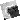
\includegraphics[width=0.9\textwidth]{rotacoes/16_alp_viz.png}
        \caption{~\texttt{vizinho}.}
    \end{subfigure}%
    \hfill%
    \begin{subfigure}{0.4\textwidth}
        \centering
        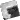
\includegraphics[width=0.9\textwidth]{rotacoes/16_alp_bil.png}
        \caption{~\texttt{bilinear}.}
    \end{subfigure}\hfill
    \\[8pt]\hfill
    \begin{subfigure}{0.4\textwidth}
        \centering
        \includegraphics[width=0.9\textwidth]{rotacoes/16_alp_bic.png}
        \caption{~\texttt{bicubica}.}
    \end{subfigure}%
    \hfill%
    \begin{subfigure}{0.4\textwidth}
        \centering
        \includegraphics[width=0.9\textwidth]{rotacoes/16_alp_lag.png}
        \caption{~\texttt{lagrange}.}
    \end{subfigure}\hfill

    \caption{Rotação de 15\textdegree{} no plano da imagem aplicada em \texttt{house16.png} ($16 \times 16$).}
    \label{fig:house16:alp}
\end{figure}

    \begin{figure}[H]
    \centering
    \begin{subfigure}{0.33\textwidth}
        \centering
        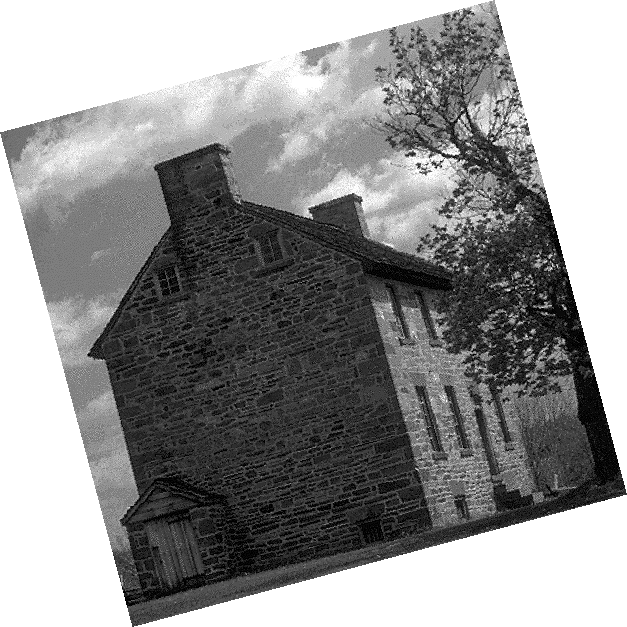
\includegraphics[width=0.9\textwidth]{rotacoes/house_alp_viz.png}
        \caption{~\texttt{vizinho}.}
    \end{subfigure}%
    \hspace{8pt}
    \begin{subfigure}{0.33\textwidth}
        \centering
        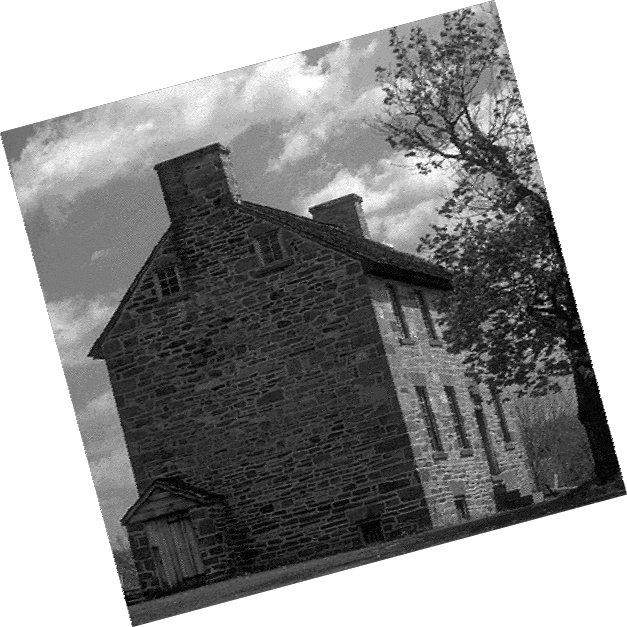
\includegraphics[width=0.9\textwidth]{rotacoes/house_alp_bil.png}
        \caption{~\texttt{bilinear}.}
    \end{subfigure}
    \\[8pt]
    \begin{subfigure}{0.33\textwidth}
        \centering
        \includegraphics[width=0.9\textwidth]{rotacoes/house_alp_bic.png}
        \caption{~\texttt{bicubica}.}
    \end{subfigure}%
    \hspace{8pt}%
    \begin{subfigure}{0.33\textwidth}
        \centering
        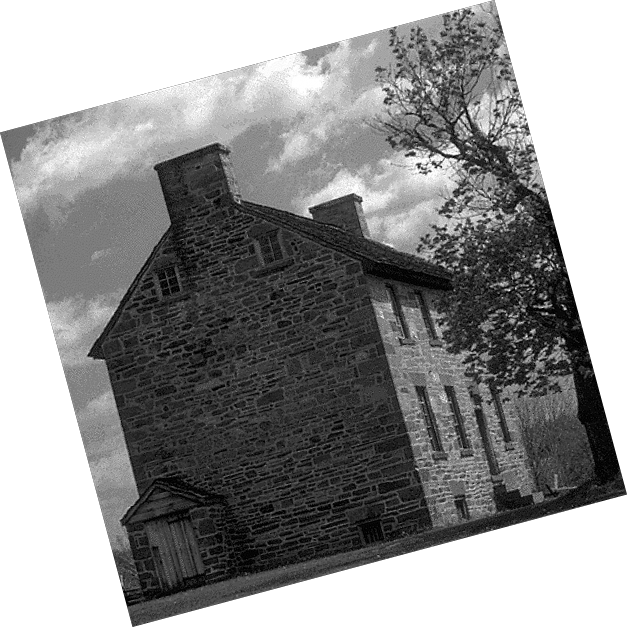
\includegraphics[width=0.9\textwidth]{rotacoes/house_alp_lag.png}
        \caption{~\texttt{lagrange}.}
    \end{subfigure}

    \caption{Rotação de 15\textdegree{} no plano da imagem aplicada em \texttt{house.png} ($512 \times 512$).}
    \label{fig:rot:house}
\end{figure}

    \begin{figure}[H]
    \centering
    \begin{subfigure}{0.3\textwidth}
        \centering
        \includegraphics[width=0.8\textwidth]{rotacoes/64_alp_viz.png}
        \caption{~\texttt{vizinho}.}
    \end{subfigure}%
    \hspace{8pt}%
    \begin{subfigure}{0.3\textwidth}
        \centering
        \includegraphics[width=0.8\textwidth]{rotacoes/64_alp_bil.png}
        \caption{~\texttt{bilinear}.}
    \end{subfigure}
    \\[8pt]
    \begin{subfigure}{0.3\textwidth}
        \centering
        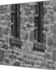
\includegraphics[width=0.8\textwidth]{rotacoes/64_alp_bic.png}
        \caption{~\texttt{bicubica}.}
    \end{subfigure}%
    \hspace{8pt}%
    \begin{subfigure}{0.3\textwidth}
        \centering
        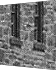
\includegraphics[width=0.8\textwidth]{rotacoes/64_alp_lag.png}
        \caption{~\texttt{lagrange}.}
    \end{subfigure}

    \caption{Rotação de -30\textdegree{} no plano da imagem aplicada em \texttt{house16.png} ($64 \times 64$).}
    \label{fig:rot:house64}
\end{figure}

\subsection{Ampliação}

\subsection{Redução}

\subsection{Reconstrução}

\subsection{Tempo de Execução}


    \section{Conclusão}

Podemos ver que a diferenças dos métodos de interpolação é grande, tanto em relação ao resultado quanto ao tempo necessário para a aplicação. Os métodos mais custosos são os que tem melhores resultados visuais, no caso as interpolações cúbica e por polinômios de Lagrange. No entanto, o método de Lagrange consegue ser melhor em várias situações, por evitar borramento da imagem, mesmo sendo bem mais eficiente.

Em algumas situações, como no caso de \hyperref[sec:escalonamento]{redução das dimensões da imagem}, a interpolação bicúbica pode ser melhor. O método pode ser melhorado ainda mais com algum filtro de frequência, como um de nitidez. Em aplicações como redes neurais, em que \textit{downsampling} é muito importante, esse método pode ser bem útil.

Em outras situações em que \textit{downsampling} também pe necessário, mas não afeta tanto o resultado, a interpolação por vizinho mais próximo pode ser mais interessante. Isso por sua eficiência, capaz de produzir imagens com 20 mega pixels em poucos segundos.


\end{document}
